\section{第6章\quad 实用微波传输线与波导}
\begin{frame}{第6章\quad 实用微波传输线与波导}
    \begin{itemize}
        \item 微波工程分析方法
              \begin{itemize}
                  \item 场论的方法
                  \item 网络的方法
              \end{itemize}
    \end{itemize}
    \begin{itemize}
        \item 传输线理论 $\Longrightarrow$ 波导
              \begin{itemize}
                  \item 当其他人或物靠近双导线时会产生较大影响。这说明,传输线与外界有能量交换,它带来的直接问题是能量损失和工作不稳定。就其原因是\textbf{开放(Open)}造成的特点
              \end{itemize}
    \end{itemize}
\end{frame}

\begin{frame}{第6章\quad 实用微波传输线与波导}
    \begin{itemize}
        \item 波导(Waveguide)构成
    \end{itemize}
    双导线两侧连续加对称$\lambda/4$支节,直到构成封闭(Closed)电路为止。如果其导线的宽度是$W$,则波导宽边
    \begin{align*}
        a=W+2\cdot \frac{\lambda}{4}=W+\frac{\lambda}{2} \\
        a\geqslant \lambda/2 或 \lambda\leqslant 2a
    \end{align*}
    这构成了波导传输的第一个约束条件 \\
    \centering
    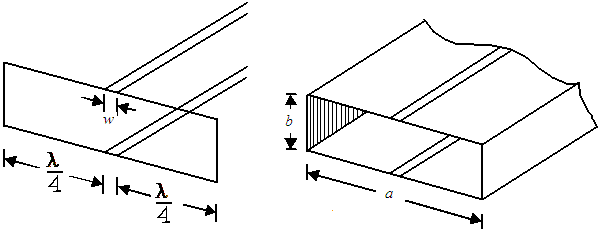
\includegraphics[width=6cm]{fig6-0.png}
\end{frame}

\begin{frame}{第6章\quad 实用微波传输线与波导}
    \begin{itemize}
        \item 波导一般解的出发点和假定条件\\
              波导一般解的出发点是频域Maxwell方程组
              \begin{align}
                  \begin{cases}
                      \nabla\times\vec{H}=\rm{j}\omega\epsilon\vec{E} \\
                      \nabla\times\vec{E}=-\rm{j}\omega\mu\vec{H}     \\
                      \nabla\cdot\vec{E}=0                            \\
                      \nabla\cdot\vec{H}=0
                  \end{cases}\label{eqn6-1}
              \end{align}
              波导假定条件
              \begin{columns}
                  \begin{column}{0.5\linewidth}
                      \begin{itemize}
                          \item 波导均匀条件:假定横截面不随$z$而变化
                          \item 媒质均匀条件:波导内部$\epsilon,\mu$均匀,波导内壁$\sigma$无限大
                          \item 无源条件:波导内$\rho,\vec{J}\equiv 0$
                          \item 无限条件:波导在$z$方向无限长
                      \end{itemize}
                  \end{column}
                  \begin{column}{0.5\linewidth}
                      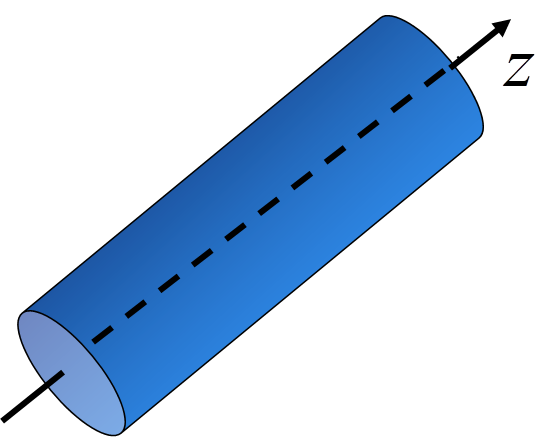
\includegraphics[width=5cm]{fig6-1.png}
                  \end{column}
              \end{columns}
    \end{itemize}
\end{frame}

\subsection{传输线的一般传输特性}
\begin{frame}{传输线的一般传输特性}
    (\ref{eqn6-1})第二式两边取旋度
    \begin{align*}
        \nabla\times\nabla\times\vec{E} & =\nabla(\nabla\cdot\vec{E})-\nabla^2\vec{E}=-\rm{j}\omega\mu\nabla\times\vec{H} \\
                                        & =\omega^2\mu\epsilon\vec{E}=k^2\vec{E}
    \end{align*}
    得到波动方程
    \begin{align}
        \begin{cases}
            \nabla^2\vec{E}+k^2\vec{E}=0 \\
            \nabla^2\vec{H}+k^2\vec{H}=0 \\
        \end{cases}\label{eqn6-2}
    \end{align}
\end{frame}

\subsection{矩形波导}
\begin{frame}{矩形波导}

\end{frame}

\subsection{圆波导}
\begin{frame}{圆波导}

\end{frame}

\subsection{同轴线}
\begin{frame}{同轴线}

\end{frame}

\subsection{平面传输线}
\begin{frame}{平面传输线}
    上世纪六十年代以来,在微波工程和微波技术上,出现了一次不小的革命,即所谓MIC(Microwave Integrated Circuit)微波集成电路——HMIC、MMIC。其特色是体积小、功能多、频带宽,但承受功率小。因此被广泛应用于接收机和小功率元件中,并都传输TEM波。\\
    作为这一革命的“过渡人物”是带状线(Stripline)。它可以看作是同轴线的变形。
\end{frame}






